% Options for packages loaded elsewhere
\PassOptionsToPackage{unicode}{hyperref}
\PassOptionsToPackage{hyphens}{url}
%
\documentclass[
  man,floatsintext]{apa6}
\usepackage{amsmath,amssymb}
\usepackage{iftex}
\ifPDFTeX
  \usepackage[T1]{fontenc}
  \usepackage[utf8]{inputenc}
  \usepackage{textcomp} % provide euro and other symbols
\else % if luatex or xetex
  \usepackage{unicode-math} % this also loads fontspec
  \defaultfontfeatures{Scale=MatchLowercase}
  \defaultfontfeatures[\rmfamily]{Ligatures=TeX,Scale=1}
\fi
\usepackage{lmodern}
\ifPDFTeX\else
  % xetex/luatex font selection
\fi
% Use upquote if available, for straight quotes in verbatim environments
\IfFileExists{upquote.sty}{\usepackage{upquote}}{}
\IfFileExists{microtype.sty}{% use microtype if available
  \usepackage[]{microtype}
  \UseMicrotypeSet[protrusion]{basicmath} % disable protrusion for tt fonts
}{}
\makeatletter
\@ifundefined{KOMAClassName}{% if non-KOMA class
  \IfFileExists{parskip.sty}{%
    \usepackage{parskip}
  }{% else
    \setlength{\parindent}{0pt}
    \setlength{\parskip}{6pt plus 2pt minus 1pt}}
}{% if KOMA class
  \KOMAoptions{parskip=half}}
\makeatother
\usepackage{xcolor}
\usepackage{graphicx}
\makeatletter
\def\maxwidth{\ifdim\Gin@nat@width>\linewidth\linewidth\else\Gin@nat@width\fi}
\def\maxheight{\ifdim\Gin@nat@height>\textheight\textheight\else\Gin@nat@height\fi}
\makeatother
% Scale images if necessary, so that they will not overflow the page
% margins by default, and it is still possible to overwrite the defaults
% using explicit options in \includegraphics[width, height, ...]{}
\setkeys{Gin}{width=\maxwidth,height=\maxheight,keepaspectratio}
% Set default figure placement to htbp
\makeatletter
\def\fps@figure{htbp}
\makeatother
\setlength{\emergencystretch}{3em} % prevent overfull lines
\providecommand{\tightlist}{%
  \setlength{\itemsep}{0pt}\setlength{\parskip}{0pt}}
\setcounter{secnumdepth}{-\maxdimen} % remove section numbering
% Make \paragraph and \subparagraph free-standing
\ifx\paragraph\undefined\else
  \let\oldparagraph\paragraph
  \renewcommand{\paragraph}[1]{\oldparagraph{#1}\mbox{}}
\fi
\ifx\subparagraph\undefined\else
  \let\oldsubparagraph\subparagraph
  \renewcommand{\subparagraph}[1]{\oldsubparagraph{#1}\mbox{}}
\fi
\newlength{\cslhangindent}
\setlength{\cslhangindent}{1.5em}
\newlength{\csllabelwidth}
\setlength{\csllabelwidth}{3em}
\newlength{\cslentryspacingunit} % times entry-spacing
\setlength{\cslentryspacingunit}{\parskip}
\newenvironment{CSLReferences}[2] % #1 hanging-ident, #2 entry spacing
 {% don't indent paragraphs
  \setlength{\parindent}{0pt}
  % turn on hanging indent if param 1 is 1
  \ifodd #1
  \let\oldpar\par
  \def\par{\hangindent=\cslhangindent\oldpar}
  \fi
  % set entry spacing
  \setlength{\parskip}{#2\cslentryspacingunit}
 }%
 {}
\usepackage{calc}
\newcommand{\CSLBlock}[1]{#1\hfill\break}
\newcommand{\CSLLeftMargin}[1]{\parbox[t]{\csllabelwidth}{#1}}
\newcommand{\CSLRightInline}[1]{\parbox[t]{\linewidth - \csllabelwidth}{#1}\break}
\newcommand{\CSLIndent}[1]{\hspace{\cslhangindent}#1}
\ifLuaTeX
\usepackage[bidi=basic]{babel}
\else
\usepackage[bidi=default]{babel}
\fi
\babelprovide[main,import]{english}
% get rid of language-specific shorthands (see #6817):
\let\LanguageShortHands\languageshorthands
\def\languageshorthands#1{}
% Manuscript styling
\usepackage{upgreek}
\captionsetup{font=singlespacing,justification=justified}

% Table formatting
\usepackage{longtable}
\usepackage{lscape}
% \usepackage[counterclockwise]{rotating}   % Landscape page setup for large tables
\usepackage{multirow}		% Table styling
\usepackage{tabularx}		% Control Column width
\usepackage[flushleft]{threeparttable}	% Allows for three part tables with a specified notes section
\usepackage{threeparttablex}            % Lets threeparttable work with longtable

% Create new environments so endfloat can handle them
% \newenvironment{ltable}
%   {\begin{landscape}\centering\begin{threeparttable}}
%   {\end{threeparttable}\end{landscape}}
\newenvironment{lltable}{\begin{landscape}\centering\begin{ThreePartTable}}{\end{ThreePartTable}\end{landscape}}

% Enables adjusting longtable caption width to table width
% Solution found at http://golatex.de/longtable-mit-caption-so-breit-wie-die-tabelle-t15767.html
\makeatletter
\newcommand\LastLTentrywidth{1em}
\newlength\longtablewidth
\setlength{\longtablewidth}{1in}
\newcommand{\getlongtablewidth}{\begingroup \ifcsname LT@\roman{LT@tables}\endcsname \global\longtablewidth=0pt \renewcommand{\LT@entry}[2]{\global\advance\longtablewidth by ##2\relax\gdef\LastLTentrywidth{##2}}\@nameuse{LT@\roman{LT@tables}} \fi \endgroup}

% \setlength{\parindent}{0.5in}
% \setlength{\parskip}{0pt plus 0pt minus 0pt}

% Overwrite redefinition of paragraph and subparagraph by the default LaTeX template
% See https://github.com/crsh/papaja/issues/292
\makeatletter
\renewcommand{\paragraph}{\@startsection{paragraph}{4}{\parindent}%
  {0\baselineskip \@plus 0.2ex \@minus 0.2ex}%
  {-1em}%
  {\normalfont\normalsize\bfseries\itshape\typesectitle}}

\renewcommand{\subparagraph}[1]{\@startsection{subparagraph}{5}{1em}%
  {0\baselineskip \@plus 0.2ex \@minus 0.2ex}%
  {-\z@\relax}%
  {\normalfont\normalsize\itshape\hspace{\parindent}{#1}\textit{\addperi}}{\relax}}
\makeatother

% \usepackage{etoolbox}
\makeatletter
\patchcmd{\HyOrg@maketitle}
  {\section{\normalfont\normalsize\abstractname}}
  {\section*{\normalfont\normalsize\abstractname}}
  {}{\typeout{Failed to patch abstract.}}
\patchcmd{\HyOrg@maketitle}
  {\section{\protect\normalfont{\@title}}}
  {\section*{\protect\normalfont{\@title}}}
  {}{\typeout{Failed to patch title.}}
\makeatother

\usepackage{xpatch}
\makeatletter
\xapptocmd\appendix
  {\xapptocmd\section
    {\addcontentsline{toc}{section}{\appendixname\ifoneappendix\else~\theappendix\fi\\: #1}}
    {}{\InnerPatchFailed}%
  }
{}{\PatchFailed}
\keywords{cognitive aging, Rescorla Wagner, spreading activation, network science, free associations, fluid intelligence, crystallized intelligence, cognitive slowing}
\usepackage{lineno}

\linenumbers
\usepackage{csquotes}
\ifLuaTeX
  \usepackage{selnolig}  % disable illegal ligatures
\fi
\IfFileExists{bookmark.sty}{\usepackage{bookmark}}{\usepackage{hyperref}}
\IfFileExists{xurl.sty}{\usepackage{xurl}}{} % add URL line breaks if available
\urlstyle{same}
\hypersetup{
  pdftitle={A network enrichment account of cognitive aging},
  pdfauthor={Thomas T. Hills1},
  pdflang={en-EN},
  pdfkeywords={cognitive aging, Rescorla Wagner, spreading activation, network science, free associations, fluid intelligence, crystallized intelligence, cognitive slowing},
  hidelinks,
  pdfcreator={LaTeX via pandoc}}

\title{A network enrichment account of cognitive aging}
\author{Thomas T. Hills\textsuperscript{1}}
\date{}


\shorttitle{Enrichment and cognitive aging}

\authornote{

This work was supported by the Alan Turing Institute and Royal Society Wolfson Research Merit Award WM160074.

Correspondence concerning this article should be addressed to Thomas T. Hills, Gibbet Hill Road, Coventry, CV4 7AL, UK. E-mail: \href{mailto:t.t.hills@warwick.ac.uk}{\nolinkurl{t.t.hills@warwick.ac.uk}}

}

\affiliation{\vspace{0.5cm}\textsuperscript{1} University of Warwick}

\abstract{%
Late-life cognitive development is associated with a decline in fluid intelligence which occurs alongside a corresponding increase in crystallized intelligence.
Theory often treats these accounts independently, seeing the former as a consequence of biological aging and the latter as a consequence of learning. What has not been fully explored is that lifelong learning may explain both accounts. This article describes a formal enrichment account that shows how a lifetime of experience encodes a cognitive representation that, when used to guide behavior, produces numerous quantitative effects commonly described for cognitive aging: with age, similarity judgments between concepts fall, free associations become less predictable (higher entropy), and free association networks produced by aggregating output across associates show patterns of declining connectivity. The enrichment account demonstrates how these behavioral outcomes arise when a general prediction error model (Rescorla-Wagner) is used to train a cognitive representation through repeated experience with a structured environment and the cognitive representation is then sampled from to produce behavior. The resulting diffusion of activity and its associated consequences is a general property of network enrichment which also speaks directly to cognitive aging. Moreover, as measures of co-activation, rising entropy and falling similarity judgments provide mechanisms for cognitive slowing, explaining declining fluid intelligence. These results help better inform mechanisms of aging and its associated pathologies by better calibrating our predictions for accounts based on atrophy and enrichment.
}



\begin{document}
\maketitle

Cognitive aging across the adult lifespan is characterized by two distinct and well-documented patterns. As individuals age, measures of working memory, processing speed, and long-term memory show performance decrements from approximately age 20, while at the same time, measures of vocabulary and other kinds of general knowledge increase (Brysbaert, Stevens, Mandera, \& Keuleers, 2016; Park \& Reuter-Lorenz, 2009; Salthouse, 2004). This distinction between the ability to solve novel problems in a fast and accurate way, called \emph{fluid intelligence}, and the quantity of one's prior knowledge, called \emph{crystallized intelligence}, is a classic division of intelligence (Cattell, 1987). This division also characteristically distinguishes the old from the young. What explains these age-related changes? Might they be explained by a single process? The evidence I provide below suggests that the answer is yes: the outcome of enriching one's cognitive representation through a lifetime of experiencing associations in the world produces an average decline in activation between any two concepts chosen at random. Before demonstrating how this effect arises, it is first useful to highlight the focal alternative accounts of aging this work addresses and to describe the behavioral effects we hope to explain.

\hypertarget{degradation-or-enrichment}{%
\section{Degradation or enrichment}\label{degradation-or-enrichment}}

Cognitive aging is a rich process with evidence supporting a wide range of phenomenology and theoretical explanations (Cao et al., 2014; Grady, Springer, Hongwanishkul, McIntosh, \& Winocur, 2006; Koen \& Rugg, 2019; Mata, Schooler, \& Rieskamp, 2007; e.g., Reuter-Lorenz \& Cappell, 2008; Spreng \& Turner, 2021; Troyer, Moscovitch, \& Winocur, 1997). Much of this work is often interpreted as supporting either degradation-based accounts (e.g., involving declining frontal lobe or executive function and neural atrophy) or enrichment-based accounts (e.g., involving adaptive consequences of lifelong learning), and sometimes both. This dichotomy between things falling apart or things coming together is well characterized by the distinction between fluid and crystallized intelligence.

Declines in fluid intelligence are often seen as independent of rising crystallized intelligence. One prominant explanation for declines in fluid intelligence is the common cause theory of age-related cognitive decline, which argues that biological aging in the brain is the source of processing speed deficits (Deary et al., 2009). The supposition is that aging is a general process of degradation, in which factors like oxidative stress and telomere shortening damage the physiological mechanisms underpinning cognitive performance. Salthouse (1992) describes some potential mechanisms as follows: ``a slower speed of transmission along single (e.g., loss of myelination) or multiple (e.g., loss of functional cells dictating circuitous linkages) pathways, or. . . delayed propagation at the connections between neural units (e.g., impairment in functioning of neurotransmitters, reduced synchronization of activation patterns)'' (p.~116). Consistent with this, percent volume of grey and white-matter declines in late life (Ge et al., 2002; Giorgio et al., 2010). Cortical thickness also declines alongside increases in cerebrospinal fluid space (Lemaitre et al., 2012). These findings are often associated with atrophy and fit with common intuitions for biological aging---as biological things fall apart, so do the cognitive counterparts which they underpin. Moreover, neuropathology---associated with posthumously verified evidence of Alzheimer's and other neurodegenerative and cerebrovascular disease---accounts for up to 40\% of the variation in late-life cognitive decline (Boyle et al., 2021). Though this leaves substantial variance in cognitive-decline unexplained, it nonetheless identifies an important correspondence between biology and cognition, especially in unhealthy aging.

Alternatively, and far more rarely, some accounts of cognitive aging have proposed an causal interdependence between the positive consequences of learning associated with crystallized intelligence and the resulting negative consequences for fluid intelligence. For example, Buchler and Reder (2007) showed using simulations that if they assumed that the number of relations between concepts increased over the lifespan this would lead to more diffuse activation between concepts, analogous to a contextual fan effect. This reproduced age-related changes in recognition and familiarity. Using a different approach, Ramscar, Hendrix, Shaoul, Milin, and Baayen (2014) demonstrated how associations would change through repeated learning. They based their work on Desrosiers and Ivison (1986) study of paired-associate learning in older adults, which found that older adults perform most poorly on stimuli that are least consistent with their prior experience. Ramscar, Sun, Hendrix, and Baayen (2017) showed that the difficulty of learning unrelated word pairs is entirely predictable from the co-occurrence frequency of those pairs in past experience. Training a Rescorla-Wagner model on typical patterns of word co-occurrences, unrelated word pairs become negatively associated over time, impairing the future learning of their association.

Still more recent work has argued for a much broader influence of age-related mental `clutter', which may arise from representational changes across the lifespan as well as changes in cognitive control at the time of encoding or retrieval (Amer, Wynn, \& Hasher, 2022). According to this account, processing deficits and the inability to filter out past experience can lead older adults to attend to too much information. This in turn creates processing difficulties when that information turns out to be irrelevant. For example, Li and Siew (2022) showed older individuals were more likely to show processing difficulties for words that changed their meaning during their lifetime. Though there is no existing formal model of clutter development, the enrichment account provided below offers one.

The different accounts describe above can be broadly categorized as degradation versus enrichment accounts, and the evidence for both is compelling. However, to what extent we subscribe to one explanation over another should largely depend on how they work and what they explain. To my knowledge, the degradation accounts have not provided formal computational mechanisms for how degradation might lead to the observed age-related changes in healthy individuals. Presumably such mechanisms could be developed and would offer useful predictions. For example, Borge-Holthoefer, Moreno, and Arenas (2011) have developed a compelling model of degradation for hyper-priming in Alzheimer's patients, but similar models for healthy aging are still needed. A key challenge for formal degradation models is that they would need to explain how degradation alters fluid intelligence but not crystallized intelligence.

On the other hand, enrichment explanations either assume more connectivity (e.g., Buchler \& Reder, 2007) or evaluate how differential experience impairs or enhances pair-wise associations (e.g., Ramscar et al., 2014). As called for elsewhere (Wulff, De Deyne, Jones, \& Mata, 2019), what is lacking in both cases is a full model of representational development and behavior across the adult lifespan that takes into account our understanding of the aging lexicon. This would represent a computational prediction for what we should expect from lifelong enrichment and what remains to be explained by degradation. This is what we hope to achieve here. To benchmark such a model, we can use a number of empirical observations made over the last decade.

\hypertarget{the-aging-lexicon-entropy-and-similarity}{%
\section{The aging lexicon, entropy, and similarity}\label{the-aging-lexicon-entropy-and-similarity}}

Several efforts to chart the mental lexicon across the lifespan have identified reproducible trends. Dubossarsky, De Deyne, and Hills (2017) asked over 8000 people, ranging in age from roughly 10 to 70, to provide three free associates to each of 420 words. With approximately 1000 people in each age group, data was aggregated within age-groups to produce networks among the 420 words with edges representing a weighted function of common associates. After removing edges below a threshold, older networks were found to have a lower average degree (number of associations per word) higher average shortest path length (greater distance between associates), and lower average clustering coefficient (the proportion of a concept's neighbors that are themselves connected). Evidence also identified a rising entropy for associations, with associates becoming less predictable across the lifespan. Both Zortea, Menegola, Villavicencio, and Salles (2014) and Wulff, De Deyne, Aeschbach, and Mata (2022) found similar patterns with varying numbers of participants and cues and with some variations based on network construction methods.

Analyses of memory search in older and younger adults also find consistent patterns of change in the aging mental lexicon. Using a semantic fluency task (``name all the animals you can think of''), Wulff, Hills, and Mata (2022) constructed lexical networks by connecting words that appeared nearby in the lists that older and younger adults produced. Older adults' produced less well-connected networks, similar to the patterns for free associations described above. Hills, Mata, Wilke, and Samanez-Larkin (2013) modeled semantic fluency data from adults across the lifespan and found that, compared with younger adults, older adults produced strings of animal names that were less predictable, one from the next. Finally, Cosgrove, Kenett, Beaty, and Diaz (2021) used percolation analysis to investigate the resilience of older adults' mental lexicons by artificially removing connections between words and found that older adults' lexicons were less resilient to decay. These findings are all suggestive of more sparse connectivity in the outputs retrieved from the mental lexicon.

Slower judgments of similarity between words are consistent with the above patterns. Wulff, Hills, et al. (2022) asked younger and older adults to judge the similarity of 77 different animals over a period of several weeks using a tablet participants took to their homes. Rating the similarity of pairs of animals on a scale from 1 to 20, they found that older adults rated animals as less similar to one another than did young adults. Again, this indicates a sparsening of the connectivity between concepts in the mental lexicon.

The above results indicate that older adults produce less predictable associations (higher entropy), lower similarity judgments, and show evidence of sparsening free association networks. These results are intuitively consistent with representational degradation: one may imagine that a sparseness in output reflects a sparseness in the underlying representation, which is in turn caused by degradation in the neural architecture that underpins it. However, without understanding what we might expect from lifelong learning, efforts to explain cognitive aging as the result of degradation may attempt to bridge an explanatory gap that does not exist. Moreover, degradation accounts may even get the causation backwards. Which is to say, if life experience gives rise to some of the primary markers of age-related cognitive decline, then so-called atrophy in physiological structure may not be the cause of age-related cognitive decline. Rather, it may be the consequence of life-long experience. As demonstrated below, by extending standard learning and retrieval models across the lifespan, we can predict all of the above effects---rising entropy, falling similarity, and sparsening free association networks---as a consequence of enrichment, without the need for assuming any additional processes associated with biological aging or degradation.

\hypertarget{the-enrichment-account}{%
\section{The enrichment account}\label{the-enrichment-account}}

The enrichment account envisions behavior as the outcome of learning relationships from the environment to develop a cognitive representation, and then using this representation to generate behavior. This follows calls from previous researchers to model not only the representation but the processes that access that representation to generate behavior (Castro \& Siew, 2020; Estes, 1975; Hills \& Kenett, 2022; Johns, Jamieson, \& Jones, 2023; Jones, Hills, \& Todd, 2015). Formally, the enrichment account involves modeling three separate components:

\begin{enumerate}
\def\labelenumi{\arabic{enumi}.}
\tightlist
\item
  \emph{Environment}: The environment presents the set of all possible associations that could be learned.
\item
  \emph{Representation}: Learning associations from the environment generates a cognitive representation. This continues to develop across the lifespan.
\item
  \emph{Behavior}: Behavior is recovery of information from the cognitive representation appropriate to the environmental context. This generates free-associations, memory search, similarity judgments, and so on.
\end{enumerate}

These stages are presented in Figure \ref{fig:Figure1} and each are explained in detail below. The R code to reproduce the environments, the learning of cognitive representations, the behavior, and all analyses and figures in this manuscript are available at \url{https://github.com/thomasthills/enrichment}.

\begin{figure}
\centering
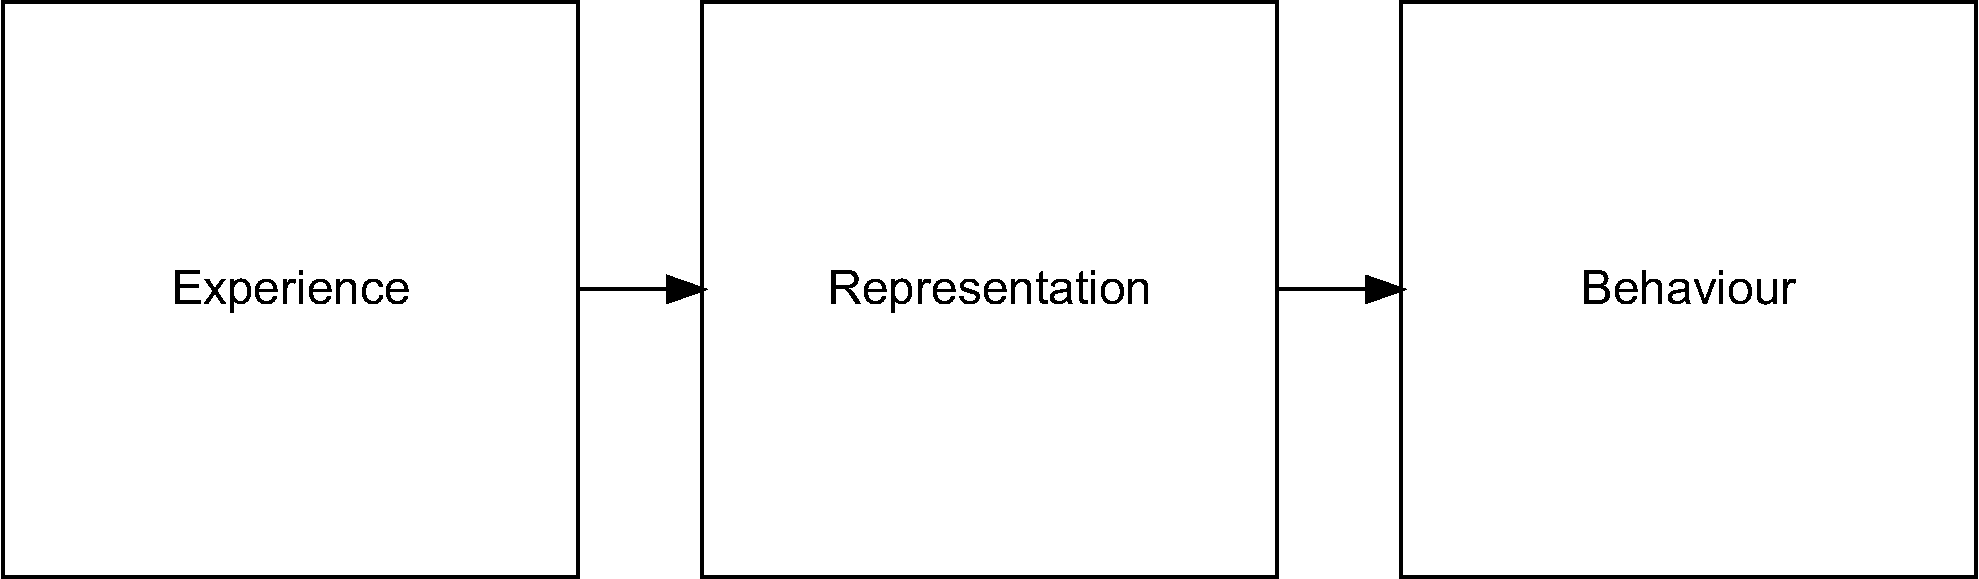
\includegraphics{Enrichment_files/figure-latex/Figure1-1.pdf}
\caption{\label{fig:Figure1}The process of translating experience with the environment into behaviour. Arrows represent processes that translate one domain into another. Learning translates experience with the environment into a cognitive representation. Additional cognitive processes then act on the representation to generate behavior.}
\end{figure}

\hypertarget{environment}{%
\subsection{Environment}\label{environment}}

The environment is represented here as network of concepts (e.g., words), with the edges (links) between concepts indicating associations that can be learned. This follows the basic idea that things in the world predict one another, and learning is here taken to address one association at a time. The qualitative pattern of behavioral results described below are not dependent on the specific network structure. To demonstrate this, I use a general framework for network construction. This is a variation of a fitness-based network model (Menczer, Fortunato, \& Davis, 2020) in which all nodes are present at the start and edges are formed using rank-based sampling. Each concept is assigned a rank, \(r\), from 1 to \(n\). Then pairs of concepts are chosen from the lexicon each with probability \(p \propto r^{-a}\) and an edge is created between them. When \(a=1\), this process produces a scale-free network, which is characterized by a long-tail in which most concepts have very few associations and a few have very many. This structure is consistent with the ubiquity of scaling laws in the cognitive sciences and the natural world (Johns \& Jones, 2010; Kello et al., 2010). Providing a useful point of comparision, when \(a=0\) the resulting network approximates a weighted Erdös-Renyi random graph, in which all nodes are connected with equal probability.

The estimate of the number of concepts people know in late life varies widely. A factor of 10 estimate is generally around 100,000, though this increases across the lifespan (Brysbaert et al., 2016). The number of relationships between concepts is limited only by the network size and the human capacity to relate them. In practice, humans report only a subset of all potential associations (De Deyne, Navarro, Perfors, Brysbaert, \& Storms, 2019; Nelson, McEvoy, \& Schreiber, 2004). For example, the number of associations people reported between the approximately 12,000 cues provided in De Deyne et al. (2019) \(0.15 \%\) of the approximately 72 million possible associations. These are unlikely to represent all possible associations in the environment or in their cognitive representation. For example, people rarely provide ``eyes'' as an associate of ``horse'', though most people probably see horses with eyes about as often as they see horses. This makes predicting the number of associations in the environment problematic. For the purposes of demonstration, a small vocabulary is used of \(n=500\) concepts. From these concepts, \(2000\) pairs are sampled (with replacement) and weighted edges are formed between them, with the weight corresponding to the number of times the pair is chosen. The edges are weighted and undirected. Figure \ref{fig:Figure2} presents two example networks and their weighted degree (strength) distributions for the different values of \(a\). The Supplementary Material demonstrates that the qualitative pattern of results presented here is not altered by substantially increasing or decreasing the number of sampled pairs.

\begin{figure}
\centering
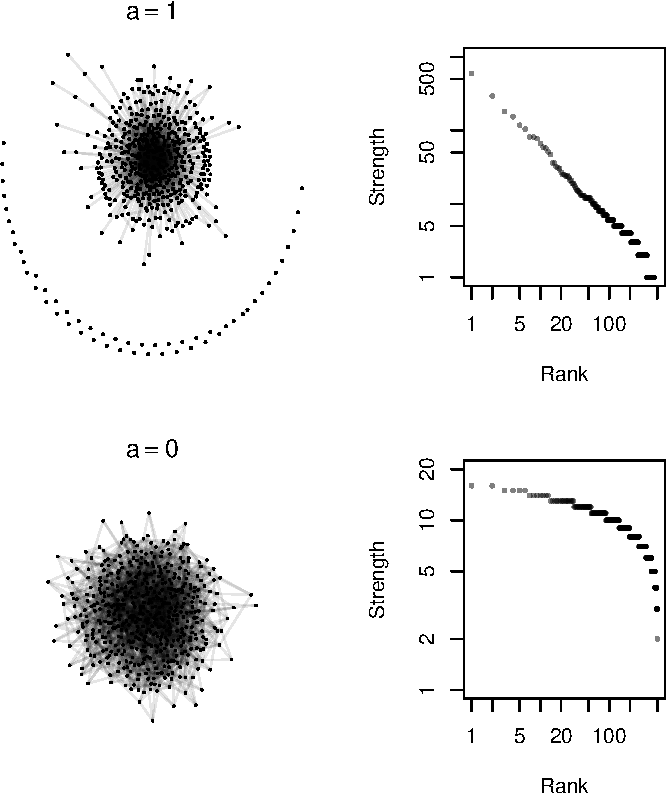
\includegraphics{Enrichment_files/figure-latex/Figure2-1.pdf}
\caption{\label{fig:Figure2}The structure of the environment for two network types: A scale-free network (\(a=1\)) and a weighted Erdös-Renyi random graph (\(a=0\)). Each network has 500 concepts (or nodes) and the weighted edges between them are the result of repeatedly sampling 2000 pairs of nodes and adding 1 to the edge weight between the pairs. The strength distributions (sum of the edge weights) are shown to help communicate the difference in the underlying structure.}
\end{figure}

\hypertarget{representation}{%
\subsection{Representation}\label{representation}}

Cognitive representations are built from experience with the environment. I use the prediction error framework set out in the Rescorla-Wagner model (Rescorla \& Wagner, 1972) to encode properties of the environment into a cognitive representation. The choice of the Rescorla-Wagner model follows the strong evidence for learning as a process of minimizing prediction error, which is a fundamental assumption among models of reinforcement learning (Dayan \& Abbott, 2005; Hoppe, Hendriks, Ramscar, \& Rij, 2022; McClelland \& Rumelhart, 1981; Sutton \& Barto, 2018). The Rescorla-Wagner model captures this phenomenology---including associative learning, blocking, inhibition, and extinction---and it is a model on which many subsequent models have been based (e.g., Sutton \& Barto, 1981). Though it is not without limitations (Miller, Barnet, \& Grahame, 1995; e.g., Yau \& McNally, 2023), these are largely irrelevant here and the Supplementary Material shows that removing a key assumption (the context cue) does not alter the results. I therefore use the model to capture the generic prediction-error process inherent in the Rescorla-Wagner design and in recognition of its extreme predictive utility (Miller et al., 1995; Roesch, Esber, Li, Daw, \& Schoenbaum, 2012; e.g., Soto, Vogel, Uribe-Bahamonde, \& Perez, 2023; Trimmer, McNamara, Houston, \& Marshall, 2012).

Formally, the Rescorla-Wagner model minimizes the prediction error between the values of an observed outcome, \(j\), and a cue predictive of that outcome, \(i\). The value associated with the outcome is \(\lambda_j\) and the value for that outcome as predicted by the cue is \(V_{i \rightarrow j}\). The prediction error is the difference between them, \((\lambda_j-V_i)\), and it is minimized following each learning event according to the following rule:

\[
\Delta V_{i \rightarrow j} = \alpha_i \beta_j (\lambda_{j} - V_{i \rightarrow j})
\]

The parameter \(\alpha_i\) corresponds to cue salience (some cues are easier to learn about than others) and \(\beta_j\) to the learning rate (some outcomes are learned about faster than others). Both \(\alpha\) and \(\beta\) values are confined to values between \(0\) and \(1\). After learning at time \(t\), the updated cue value is

\[
V_{i \rightarrow j, t+1} = V_{i \rightarrow j, t} + \Delta V_{i \rightarrow j, t}
\]

Thus, with repeated experience, \(V_{i \rightarrow j}\) will approach the observed value \(\lambda_j\). This follows exactly the formalization set out in prior work (Ramscar et al., 2017; Rescorla \& Wagner, 1972).

The cognitive representation is formed by applying the Rescorla-Wagner model to the environment in the following way. Each learning event randomly samples a relationship (i.e., edge) from the environment in proportion to its weight (the number of times it is represented in the environment). Of the two concepts associated with the relationship, one is randomly assigned as the cue and the other as the outcome. The representation is then updated according to the Rescorla-Wagner model. Here, we let all outcomes be equivalent and associated with \(\alpha=1\) and \(\lambda=1\). To demonstrate that the qualitative results are not dependent on the precise learning values, \(\beta\) is varied from \(.01\) to \(.1\) in the manuscript, and from \(.1\) to \(.5\) in the Supplemental material, covering the range of values common to this model in the literature cited above.

To simulate development, learning occurs in 4 epochs each with 200 learning trials. The precise number of learning trials per epoch is unrelated to the qualitative pattern of results, and is explored further in the Supplemental Material. Figure \ref{fig:Figure3} provides examples of two learning representations over the four epochs for the different network types (\(a=0\) and \(a=1\)) and varying values of \(\beta\).

\begin{figure}
\centering
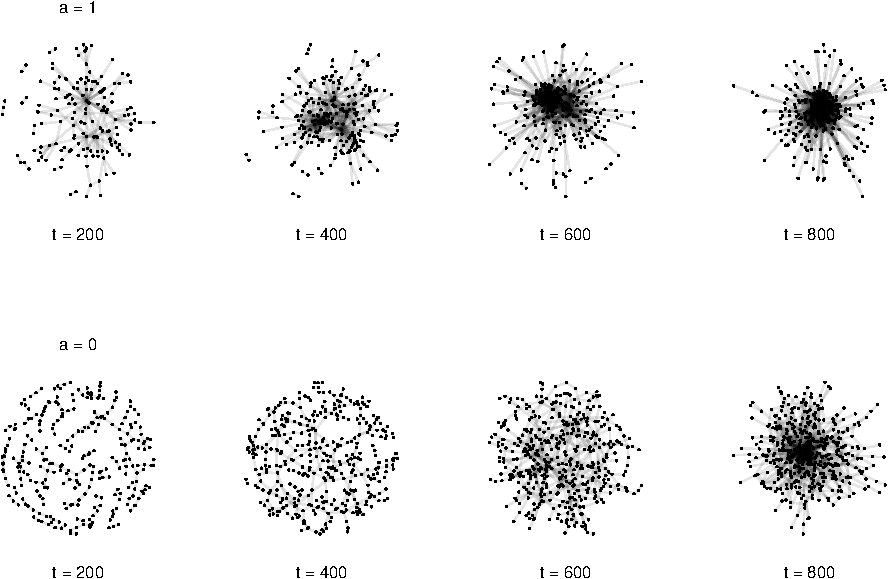
\includegraphics{Enrichment_files/figure-latex/Figure3-1.pdf}
\caption{\label{fig:Figure3}Examples of the growing mental lexicon resulting from training a Rescorla-Wagner model on the network types shown in Figure 2. Training occurs in 200 event epochs, with edges from the environment sampled in proportion to their weight. Nodes represent individual concepts and edges represent learned associations.}
\end{figure}

\hypertarget{results-behavior}{%
\section{Results: Behavior}\label{results-behavior}}

The stylized facts associated with cognitive aging are rising entropy, a reduction in pairwise similarity judgments, and changes in the structure of the free association network. Each of these is recovered from the representation as described below. In each case, environments are constructed independently 1000 times and then learning occurs over 4 epochs of 200 trials each.

\hypertarget{rising-entropy}{%
\subsubsection{Rising entropy}\label{rising-entropy}}

Rising entropy refers to the reduction in the predictability of free association targets as individuals age (Dubossarsky et al., 2017). We can measure this using \emph{Shannon's information entropy}. This measures the surprisingness of associates given the cue. If a cue has only a few strong associations, any given associate will be less surprising than if it has many equally weighted associations. Because the output of Rescorla-Wagner learning is a weighted edge, we can compute this for every cue in the network representation as follows:

\[
H = -\sum_{i=1}^{k}  p_i log(p_i)
\]

Here, \(p_i\) is the proportion of the weight along edge \(i\) for all \(k\) edges for that cue. That is, \(p_i = \frac{w_i}{\sum_k w_k}\). The entropy for the network reported below is the mean across all cues. This is taken here to represent the long-term entropy of persons producing repeated associations for each cue.

The result of this computation is shown in Figure \ref{fig:Figure4}. For various network constructions and learning rates, the results consistently show that entropy rises with increased learning, following that observed in Dubossarsky et al. (2017). In addition, entropy is higher in the scale-free network than in the weighted Erdös-Renyi random graph.

\hypertarget{falling-similarity}{%
\subsubsection{Falling similarity}\label{falling-similarity}}

To simulate similarity judgments, we can create a measure of co-activation between cues. To do this, we allow spreading activation to leave one node and measure activation at the other node, \(A_{j \rightarrow k}\). This allows us to measure the extent to which one word co-activates the other. Doing this for both cues, we take similarity as the summed co-activation.

\[
S = A_{j \rightarrow k} + A_{j \rightarrow k}
\]

We measure this similarity for a random selection of 20 concept pairs in the representation, all of which are learned during the first epoch of learning. This ensures that individuals at each age (epoch) have experience with the concepts.

The result of this computation is shown in Figure \ref{fig:Figure4}. For various network constructions and learning rates, the results consistently show that similarity judgments fall with increased learning, following that found in Wulff et al. (2019). In addition, similarity is smaller for the scale-free network than the Erdös-Renyi random graph.

\begin{figure}

{\centering 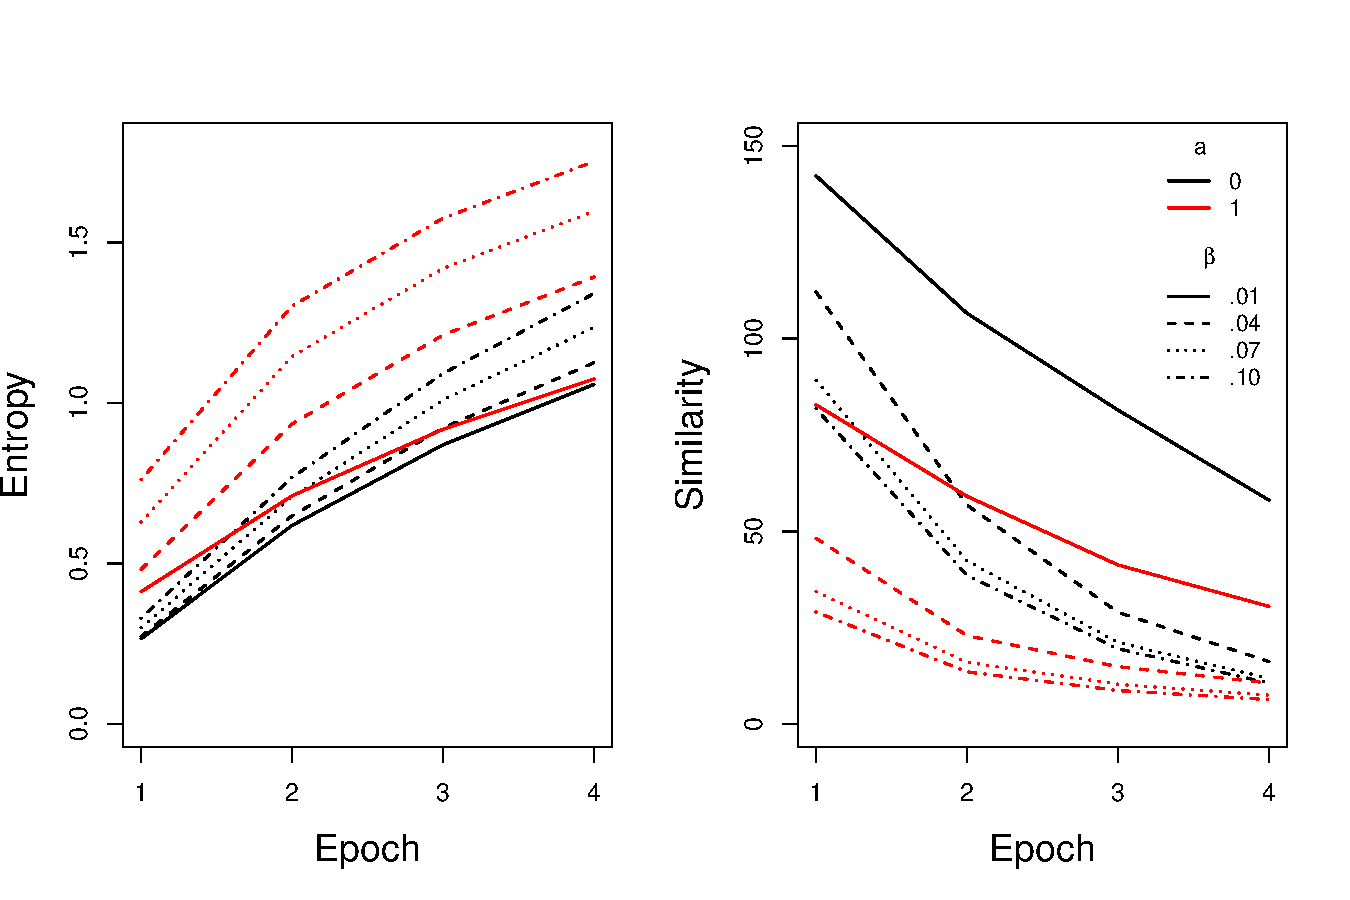
\includegraphics[width=1\linewidth]{EntropySim1000.01to.1} 

}

\caption{Entropy and similarity measures computed from the cognitive representation at different epochs of development.}\label{fig:Figure4}
\end{figure}

\hypertarget{sparsening-free-association-networks}{%
\subsubsection{Sparsening free association networks}\label{sparsening-free-association-networks}}

As noted above, Dubossarsky et al. (2017) and others found that free association networks collected across the adult lifespan showed patterns of decreasing network degree, increasing average shortest path length, and decreasing clustering coefficient. We simulate this on the cognitive representations across the four epochs as follows. For each cognitive representation, we simulate 10 participants who retrieve 3 associates from each of 30 cues. The three associates are sampled without replacement for each participant and each cue is sampled in proportion to the associative strength encoded in the cognitive representation, i.e., the output from the Rescorla-Wagner training epochs. Negative association strengths are set to 0. This produces a cue by associate matrix, with each cell indicating the number of times each associate was produced in response to each cue. From this matrix, cue-by-cue similarities are computed using cosine similarity of their corresponding associate vectors. To transform these into unweighted and undirected networks, the median cue-by-cue similarity is computed across all epochs and, for each age, cue similarities below this median value are set to 0, and all other values are set to 1. This matrix is then transformed into a network on which degree (the number of connections), average shortest path length (the shortest number of edges between cues), and clustering coefficient (the proportion of a node's neighbors that are themselves connected) are computed. This entire process is repeated for 1000 different initial starting environments. The results are shown in Figure \ref{fig:Figure5}. The results follow the pattern found by Dubossarsky et al. (2017) and others.

\begin{figure}

{\centering 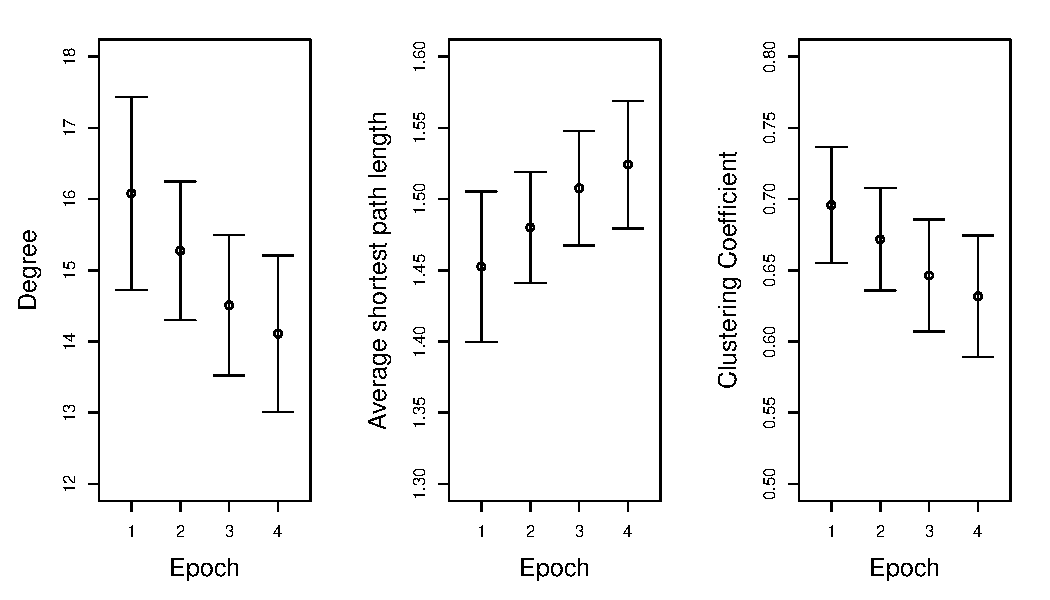
\includegraphics[width=1\linewidth]{NetworkAssociations1000} 

}

\caption{The degree, average shortest path length, and clustering coefficient for networks of associations across the lifespan. Simulations were repeated for learning cognitive representations in 1000 different environments ($a=1$) with four training epochs each of 200 learning events each($beta=.1$). Representations were then each sampled from by 10 simulated participants who each retrieved 3 associates for each of 30 cues with probability proportional to the associative strengths output from the Rescorla-Wagner training epochs. The cosine similarity of cues was then computed from the cue by association matrix to produce associative networks for each epoch. These networks were then thresholded separately for each learning environment by the median similarity value across all ages. Error bars indicate one standard deviation. Results are consistent with Dubossarsky et al., 2017.}\label{fig:Figure5}
\end{figure}

\hypertarget{discussion}{%
\section{Discussion}\label{discussion}}

Aging is marked by complex and multi-faceted phenomenology. The enrichment account provided here demonstrates that a subset of this phenomenology is predicted by cognitive enrichment. Specifically, the enrichment account demonstrates how learning enriches the cognitive representation and then, using various processes, gives rise to behavior commonly associated with cognitive aging. In particular, enrichment reproduces rising entropy, falling similarity judgments, and a sparsening of the free association network across the lifespan.

The enrichment account is not meant to be a complete explanation of cognitive aging. Rather, like any model, it puts guardrails on our ignorance. It does this by showing how many of the behaviors that might be intuitively interpreted as evidence of cognitive and neural degradation are straightforward outcomes of learning. Whereas we might have suspected degradation, enrichment may be the more likely candidate, especially given that we know enrichment is already occurring in association with crystallized intelligence. Moreover, degradation can produce the opposite effect. Borge-Holthoefer et al. (2011) used degradation \emph{not} to demonstrate diffusion of activation and greater slowing, but rather to demonstrate an increasing of activation between associates, producing hyper-priming, a well-documented behavior in patients with Alzheimer's Disease. Nonetheless, the patterns of biological and neural change outlined in the introduction are themselves data, and any full account of cognitive aging must take this evidence into account. Ideally, we want understand how these changes in neural architecture interact with enrichment to produce the behavioral variation that we see. With respect to parsimony, enrichment may be sufficient to explain how fluid intelligence might change as a result of changes in crystallized intelligence (as opposed to treating each independently), but our theories must also be parsimonious with respect to observed changes in the underlying neural architecture.

The enrichment account is incomplete for several other reasons as well. One key extension is that lifelong experience with language follows Herdan-Heap's law (Brysbaert et al., 2016). Herdan-Heaps' law is the observation that the number of new word types is an increasing function of the number of word tokens, and this appears to be true for human experience with language as well. This is easily added to the enrichment account by allowing the environment to grow over time. Future work should investigate various implications of this addition. A further limitation is that the enrichment account is not meant to characterize child development, which has special developmental features of its own. For example, early vocabulary acquisition is driven by a variety of processes including semantics, phonology, social pragmatics, and perceptual features (Ciaglia, Stella, \& Kennington, 2023; Engelthaler \& Hills, 2017; Fourtassi, Bian, \& Frank, 2020; Jiménez \& Hills, 2022; Yu, Suanda, \& Smith, 2019). This different pattern of acquisition may extend into young adulthood, possibly as a result of standardized formal education (Dubossarsky et al., 2017). Extending our understanding of the development of the cognitive representation from early childhood to late life remains for future work.

Despite these limitations, the fundamental mechanism of the enrichment account is supported empirically. For example, the fan effect demonstrates that learning many relationships with a target concept reduces the speed of accessing any one of those relationships (Anderson \& Reder, 1999). This diffusion of activation is a general and well-understood outcome of spreading activation or random walker models (Abbott, Austerweil, \& Griffiths, 2015; Siew, 2019). Activation follows pathways and the more pathways there are the less targeted the activation. In addition, one can see this effect in natural experiments: Ramscar et al. (2017) showed that individuals with more language experience (native speakers) were more impaired in paired-associative learning in that language than age-matched individuals with less experience (second language learners). This suggests the effect is not about age, but about enrichment.

We also know that external clutter influences processing speed in older adults more strongly than young adults (Amer et al., 2022; McCarley, Yamani, Kramer, \& Mounts, 2012). This is consistent with higher conceptual entropy creating a more level-playing field for competition. If there is greater associative competition in older adults, because the associative entropy is higher, then older adults will suffer more from clutter in internal and external processing. This may explain the enhanced variability in resting-state brain synchronization among older adults (Jauny, Eustache, \& Hinault, 2022). However, because external cues gain their relevance via their encoded associations in memory (Easdale, Le Pelley, \& Beesley, 2019), this may also explain the impact of external clutter. The attentional contribution to clutter on aging memory, as elegantly described by Amer et al. (2022), could therefore be a consequence of enrichment: the activation strengths associated with extraneous and potentially irrelevant information have a greater relative competitive advantage in individuals with more enriched representations, making older individuals more susceptible to internal and external distractions.

One challenge to the enrichment account is that individuals with higher education and occupational attainment are less likely to experience late-life cognitive decline (Lövdén, Fratiglioni, Glymour, Lindenberger, \& Tucker-Drob, 2020; Stern et al., 1994). This is known to be partially a consequence of compensation accorded by skills or strategic repertoires, what is called cognitive reserve (Scarmeas \& Stern, 2003). Additionally, however, there is ample evidence that differences in cognitive skills emerge early in life, prior to education, and therefore lay the foundation for educational attainment later in life (Deary, Whiteman, Starr, Whalley, \& Fox, 2004; Lövdén et al., 2020). If differences in processing speed at an early age influence educational attainment at a later age, then slowing later as a consequence of education will be confounded by early differences in processing. Early processing advantages may not be a result of experience at all. Brain volume is correlated with IQ (Pietschnig, Gerdesmann, Zeiler, \& Voracek, 2022) and is strongly heritable (Peper, Brouwer, Boomsma, Kahn, \& Hulshoff Pol, 2007). Furthermore, measures of `brain age' in late life are well-predicted by indicators present in early life (Vidal-Pineiro et al., 2021). Nonetheless, if we believe that formal education (or occupational attainment) is an indicator of increased associative density (not just in quality, but quantity), then an ideal test might be to investigate twins who differ in educational enrichment and are then evaluated on age-related cognitive decline. The Ramscar et al. (2017) study on age-matched bilinguals and monolinguals is another approach. What kinds of education matter for enrichment is an open question. Is rewatching the 11 seasons of the 1970s TV series M*A*S*H (approximately 125 hours runtime) different from reading the complete works of Gabriel Garcia Marquez for the first time? If enrichment is about the variety of associations, and not the quality of associations (if such quality could be objectively measured), then the difference may not matter.

\newpage

\hypertarget{references}{%
\section{References}\label{references}}

\hypertarget{refs}{}
\begin{CSLReferences}{1}{0}
\leavevmode\vadjust pre{\hypertarget{ref-abbott2015random}{}}%
Abbott, J. T., Austerweil, J. L., \& Griffiths, T. L. (2015). Random walks on semantic networks can resemble optimal foraging. \emph{Psychological Review}, \emph{122}(3), 558--569.

\leavevmode\vadjust pre{\hypertarget{ref-amer2022cluttered}{}}%
Amer, T., Wynn, J. S., \& Hasher, L. (2022). Cluttered memory representations shape cognition in old age. \emph{Trends in Cognitive Sciences}, \emph{26}(3), 255--267.

\leavevmode\vadjust pre{\hypertarget{ref-anderson1999fan}{}}%
Anderson, J. R., \& Reder, L. M. (1999). The fan effect: New results and new theories. \emph{Journal of Experimental Psychology: General}, \emph{128}(2), 186.

\leavevmode\vadjust pre{\hypertarget{ref-BorgeHolthoefer:2011bg}{}}%
Borge-Holthoefer, J., Moreno, Y., \& Arenas, A. (2011). {Modeling abnormal priming in Alzheimer's patients with a free association network}. \emph{PLoS ONE}, \emph{6}(8), e22651.

\leavevmode\vadjust pre{\hypertarget{ref-boyle2021degree}{}}%
Boyle, P. A., Wang, T., Yu, L., Wilson, R. S., Dawe, R., Arfanakis, K., \ldots{} Bennett, D. A. (2021). To what degree is late life cognitive decline driven by age-related neuropathologies? \emph{Brain}, \emph{144}(7), 2166--2175.

\leavevmode\vadjust pre{\hypertarget{ref-brysbaert2016many}{}}%
Brysbaert, M., Stevens, M., Mandera, P., \& Keuleers, E. (2016). How many words do we know? Practical estimates of vocabulary size dependent on word definition, the degree of language input and the participant's age. \emph{Frontiers in Psychology}, \emph{7}(1116), 1--11.

\leavevmode\vadjust pre{\hypertarget{ref-buchler2007modeling}{}}%
Buchler, N. E., \& Reder, L. M. (2007). Modeling age-related memory deficits: A two-parameter solution. \emph{Psychology and Aging}, \emph{22}(1), 104.

\leavevmode\vadjust pre{\hypertarget{ref-cao2014topological}{}}%
Cao, M., Wang, J.-H., Dai, Z.-J., Cao, X.-Y., Jiang, L.-L., Fan, F.-M., et al.others. (2014). Topological organization of the human brain functional connectome across the lifespan. \emph{Developmental Cognitive Neuroscience}, \emph{7}, 76--93.

\leavevmode\vadjust pre{\hypertarget{ref-castro2020contributions}{}}%
Castro, N., \& Siew, C. S. (2020). Contributions of modern network science to the cognitive sciences: Revisiting research spirals of representation and process. \emph{Proceedings of the Royal Society A}, \emph{476}(2238), 20190825.

\leavevmode\vadjust pre{\hypertarget{ref-cattell1987intelligence}{}}%
Cattell, R. B. (1987). \emph{Intelligence: Its structure, growth and action}. Elsevier.

\leavevmode\vadjust pre{\hypertarget{ref-ciaglia2023investigating}{}}%
Ciaglia, F., Stella, M., \& Kennington, C. (2023). Investigating preferential acquisition and attachment in early word learning through cognitive, visual and latent multiplex lexical networks. \emph{Physica A: Statistical Mechanics and Its Applications}, \emph{612}, 128468.

\leavevmode\vadjust pre{\hypertarget{ref-cosgrove2021quantifying}{}}%
Cosgrove, A. L., Kenett, Y. N., Beaty, R. E., \& Diaz, M. T. (2021). Quantifying flexibility in thought: The resiliency of semantic networks differs across the lifespan. \emph{Cognition}, \emph{211}, 104631.

\leavevmode\vadjust pre{\hypertarget{ref-dayan2005theoretical}{}}%
Dayan, P., \& Abbott, L. F. (2005). \emph{Theoretical neuroscience: Computational and mathematical modeling of neural systems}. MIT Press.

\leavevmode\vadjust pre{\hypertarget{ref-de2019small}{}}%
De Deyne, S., Navarro, D. J., Perfors, A., Brysbaert, M., \& Storms, G. (2019). {The {``Small World of Words''} English word association norms for over 12,000 cue words}. \emph{Behavior Research Methods}, \emph{51}(3), 987--1006.

\leavevmode\vadjust pre{\hypertarget{ref-deary2009age}{}}%
Deary, I. J., Corley, J., Gow, A. J., Harris, S. E., Houlihan, L. M., Marioni, R. E., \ldots{} Starr, J. M. (2009). Age-associated cognitive decline. \emph{British Medical Bulletin}, \emph{92}(1), 135--152.

\leavevmode\vadjust pre{\hypertarget{ref-deary2004impact}{}}%
Deary, I. J., Whiteman, M. C., Starr, J. M., Whalley, L. J., \& Fox, H. C. (2004). The impact of childhood intelligence on later life: Following up the scottish mental surveys of 1932 and 1947. \emph{Journal of Personality and Social Psychology}, \emph{86}(1), 130.

\leavevmode\vadjust pre{\hypertarget{ref-desrosiers1986paired}{}}%
Desrosiers, G., \& Ivison, D. (1986). Paired associate learning: Normative data for differences between high and low associate word pairs. \emph{Journal of Clinical and Experimental Neuropsychology}, \emph{8}(6), 637--642.

\leavevmode\vadjust pre{\hypertarget{ref-dubossarsky2017quantifying}{}}%
Dubossarsky, H., De Deyne, S., \& Hills, T. (2017). Quantifying the structure of free association networks across the life span. \emph{Developmental Psychology}, \emph{53}(8), 1560--1570.

\leavevmode\vadjust pre{\hypertarget{ref-easdale2019onset}{}}%
Easdale, L. C., Le Pelley, M. E., \& Beesley, T. (2019). The onset of uncertainty facilitates the learning of new associations by increasing attention to cues. \emph{Quarterly Journal of Experimental Psychology}, \emph{72}(2), 193--208.

\leavevmode\vadjust pre{\hypertarget{ref-engelthaler2017feature}{}}%
Engelthaler, T., \& Hills, T. (2017). Feature biases in early word learning: Network distinctiveness predicts age of acquisition. \emph{Cognitive Science}, \emph{41}, 120--140.

\leavevmode\vadjust pre{\hypertarget{ref-estes1975some}{}}%
Estes, W. (1975). Some targets for mathematical psychology. \emph{Journal of Mathematical Psychology}, \emph{12}(3), 263--282.

\leavevmode\vadjust pre{\hypertarget{ref-fourtassi2020growth}{}}%
Fourtassi, A., Bian, Y., \& Frank, M. C. (2020). The growth of children's semantic and phonological networks: Insight from 10 languages. \emph{Cognitive Science}, \emph{44}(7), e12847.

\leavevmode\vadjust pre{\hypertarget{ref-ge2002age}{}}%
Ge, Y., Grossman, R. I., Babb, J. S., Rabin, M. L., Mannon, L. J., \& Kolson, D. L. (2002). Age-related total gray matter and white matter changes in normal adult brain. Part i: Volumetric MR imaging analysis. \emph{American Journal of Neuroradiology}, \emph{23}(8), 1327--1333.

\leavevmode\vadjust pre{\hypertarget{ref-giorgio2010age}{}}%
Giorgio, A., Santelli, L., Tomassini, V., Bosnell, R., Smith, S., De Stefano, N., \& Johansen-Berg, H. (2010). Age-related changes in grey and white matter structure throughout adulthood. \emph{Neuroimage}, \emph{51}(3), 943--951.

\leavevmode\vadjust pre{\hypertarget{ref-grady2006age}{}}%
Grady, C. L., Springer, M. V., Hongwanishkul, D., McIntosh, A. R., \& Winocur, G. (2006). Age-related changes in brain activity across the adult lifespan. \emph{Journal of Cognitive Neuroscience}, \emph{18}(2), 227--241.

\leavevmode\vadjust pre{\hypertarget{ref-hills2022mind}{}}%
Hills, T., \& Kenett, Y. N. (2022). Is the mind a network? Maps, vehicles, and skyhooks in cognitive network science. \emph{Topics in Cognitive Science}, \emph{14}(1), 189--208.

\leavevmode\vadjust pre{\hypertarget{ref-hills2013mechanisms}{}}%
Hills, T., Mata, R., Wilke, A., \& Samanez-Larkin, G. R. (2013). Mechanisms of age-related decline in memory search across the adult life span. \emph{Developmental Psychology}, \emph{49}(12), 2396--2404.

\leavevmode\vadjust pre{\hypertarget{ref-hoppe2022exploration}{}}%
Hoppe, D. B., Hendriks, P., Ramscar, M., \& Rij, J. van. (2022). An exploration of error-driven learning in simple two-layer networks from a discriminative learning perspective. \emph{Behavior Research Methods}, \emph{54}(5), 2221--2251.

\leavevmode\vadjust pre{\hypertarget{ref-jauny2022connectivity}{}}%
Jauny, G., Eustache, F., \& Hinault, T. (2022). Connectivity dynamics and cognitive variability during aging. \emph{Neurobiology of Aging}, \emph{118}, 99--105.

\leavevmode\vadjust pre{\hypertarget{ref-jimenez2022semantic}{}}%
Jiménez, E., \& Hills, T. (2022). Semantic maturation during the comprehension-expression gap in late and typical talkers. \emph{Child Development}, \emph{93}(6), 1727--1743.

\leavevmode\vadjust pre{\hypertarget{ref-johns2023scalable}{}}%
Johns, B. T., Jamieson, R. K., \& Jones, M. N. (2023). {Scalable cognitive modelling: Putting Simon's (1969) ant back on the beach.} \emph{Canadian Journal of Experimental Psychology/Revue Canadienne de Psychologie Exp{é}rimentale}, \emph{77}(3), 185--201.

\leavevmode\vadjust pre{\hypertarget{ref-johns2010evaluating}{}}%
Johns, B. T., \& Jones, M. N. (2010). Evaluating the random representation assumption of lexical semantics in cognitive models. \emph{Psychonomic Bulletin \& Review}, \emph{17}, 662--672.

\leavevmode\vadjust pre{\hypertarget{ref-jones2015hidden}{}}%
Jones, M. N., Hills, T., \& Todd, P. M. (2015). Hidden processes in structural representations: A reply to abbott, austerweil, and griffiths (2015). \emph{Psychological Review}, \emph{122}(3), 570--574.

\leavevmode\vadjust pre{\hypertarget{ref-kello2010ga}{}}%
Kello, C. T., Brown, G. D. A., Ferrer-i-Cancho, R., Holden, J. G., Linkenkaer-Hansen, K., Rhodes, T., \& Van Orden, G. C. (2010). {Scaling laws in cognitive sciences}. \emph{Trends in Cognitive Sciences}, \emph{14}(5), 223--232.

\leavevmode\vadjust pre{\hypertarget{ref-koen2019neural}{}}%
Koen, J. D., \& Rugg, M. D. (2019). Neural dedifferentiation in the aging brain. \emph{Trends in Cognitive Sciences}, \emph{23}(7), 547--559.

\leavevmode\vadjust pre{\hypertarget{ref-lemaitre2012normal}{}}%
Lemaitre, H., Goldman, A. L., Sambataro, F., Verchinski, B. A., Meyer-Lindenberg, A., Weinberger, D. R., \& Mattay, V. S. (2012). Normal age-related brain morphometric changes: Nonuniformity across cortical thickness, surface area and gray matter volume? \emph{Neurobiology of Aging}, \emph{33}(3), 617--e1.

\leavevmode\vadjust pre{\hypertarget{ref-li2022diachronic}{}}%
Li, Y., \& Siew, C. S. (2022). Diachronic semantic change in language is constrained by how people use and learn language. \emph{Memory \& Cognition}, \emph{50}(6), 1284--1298.

\leavevmode\vadjust pre{\hypertarget{ref-lovden2020education}{}}%
Lövdén, M., Fratiglioni, L., Glymour, M. M., Lindenberger, U., \& Tucker-Drob, E. M. (2020). Education and cognitive functioning across the life span. \emph{Psychological Science in the Public Interest}, \emph{21}(1), 6--41.

\leavevmode\vadjust pre{\hypertarget{ref-mata2007aging}{}}%
Mata, R., Schooler, L. J., \& Rieskamp, J. (2007). The aging decision maker: Cognitive aging and the adaptive selection of decision strategies. \emph{Psychology and Aging}, \emph{22}(4), 796.

\leavevmode\vadjust pre{\hypertarget{ref-mccarley2012age}{}}%
McCarley, J. S., Yamani, Y., Kramer, A. F., \& Mounts, J. R. (2012). Age, clutter, and competitive selection. \emph{Psychology and Aging}, \emph{27}(3), 616.

\leavevmode\vadjust pre{\hypertarget{ref-mcclelland1981interactive}{}}%
McClelland, J. L., \& Rumelhart, D. E. (1981). An interactive activation model of context effects in letter perception: I. An account of basic findings. \emph{Psychological Review}, \emph{88}(5), 375--407.

\leavevmode\vadjust pre{\hypertarget{ref-menczer2020first}{}}%
Menczer, F., Fortunato, S., \& Davis, C. A. (2020). \emph{A first course in network science}. Cambridge University Press.

\leavevmode\vadjust pre{\hypertarget{ref-miller1995assessment}{}}%
Miller, R. R., Barnet, R. C., \& Grahame, N. J. (1995). Assessment of the rescorla-wagner model. \emph{Psychological Bulletin}, \emph{117}(3), 363.

\leavevmode\vadjust pre{\hypertarget{ref-nelson2004university}{}}%
Nelson, D. L., McEvoy, C. L., \& Schreiber, T. A. (2004). {The University of South Florida free association, rhyme, and word fragment norms}. \emph{Behavior Research Methods, Instruments, \& Computers}, \emph{36}(3), 402--407.

\leavevmode\vadjust pre{\hypertarget{ref-park2009adaptive}{}}%
Park, D. C., \& Reuter-Lorenz, P. (2009). The adaptive brain: Aging and neurocognitive scaffolding. \emph{Annual Review of Psychology}, \emph{60}, 173--196.

\leavevmode\vadjust pre{\hypertarget{ref-peper2007genetic}{}}%
Peper, J. S., Brouwer, R. M., Boomsma, D. I., Kahn, R. S., \& Hulshoff Pol, H. E. (2007). Genetic influences on human brain structure: A review of brain imaging studies in twins. \emph{Human Brain Mapping}, \emph{28}(6), 464--473.

\leavevmode\vadjust pre{\hypertarget{ref-pietschnig2022differing}{}}%
Pietschnig, J., Gerdesmann, D., Zeiler, M., \& Voracek, M. (2022). Of differing methods, disputed estimates and discordant interpretations: The meta-analytical multiverse of brain volume and IQ associations. \emph{Royal Society Open Science}, \emph{9}(5), 211621.

\leavevmode\vadjust pre{\hypertarget{ref-ramscar2014myth}{}}%
Ramscar, M., Hendrix, P., Shaoul, C., Milin, P., \& Baayen, H. (2014). The myth of cognitive decline: Non-linear dynamics of lifelong learning. \emph{Topics in Cognitive Science}, \emph{6}(1), 5--42.

\leavevmode\vadjust pre{\hypertarget{ref-ramscar2017mismeasurement}{}}%
Ramscar, M., Sun, C. C., Hendrix, P., \& Baayen, H. (2017). The mismeasurement of mind: Life-span changes in paired-associate-learning scores reflect the {``cost''} of learning, not cognitive decline. \emph{Psychological Science}, \emph{28}(8), 1171--1179.

\leavevmode\vadjust pre{\hypertarget{ref-rescorla1972theory}{}}%
Rescorla, R. A., \& Wagner, A. R. (1972). {A theory of Pavlovian conditioning: Variations in the effectiveness of reinforcement and non-reinforcement}. In A. H. Prokasy (Ed.), \emph{Classical conditioning II: Current research and theory} (pp. 64--69). Appleton-Century-Crofts.

\leavevmode\vadjust pre{\hypertarget{ref-reuter2008neurocognitive}{}}%
Reuter-Lorenz, P. A., \& Cappell, K. A. (2008). Neurocognitive aging and the compensation hypothesis. \emph{Current Directions in Psychological Science}, \emph{17}(3), 177--182.

\leavevmode\vadjust pre{\hypertarget{ref-roesch2012surprise}{}}%
Roesch, M. R., Esber, G. R., Li, J., Daw, N. D., \& Schoenbaum, G. (2012). Surprise! Neural correlates of pearce--hall and rescorla--wagner coexist within the brain. \emph{European Journal of Neuroscience}, \emph{35}(7), 1190--1200.

\leavevmode\vadjust pre{\hypertarget{ref-salthouse2013mechanisms}{}}%
Salthouse, T. A. (1992). \emph{Mechanisms of age-cognition relations in adulthood}. Lawrence Erlbaum Associates, Inc.

\leavevmode\vadjust pre{\hypertarget{ref-Salthouse:2004is}{}}%
Salthouse, T. A. (2004). {What and when of cognitive aging}. \emph{Current Directions in Psychological Science}, \emph{13}(4), 140--144.

\leavevmode\vadjust pre{\hypertarget{ref-scarmeas2003cognitive}{}}%
Scarmeas, N., \& Stern, Y. (2003). Cognitive reserve and lifestyle. \emph{Journal of Clinical and Experimental Neuropsychology}, \emph{25}(5), 625--633.

\leavevmode\vadjust pre{\hypertarget{ref-siew2019spreadr}{}}%
Siew, C. S. (2019). {spreadr: An R package to simulate spreading activation in a network}. \emph{Behavior Research Methods}, \emph{51}(2), 910--929.

\leavevmode\vadjust pre{\hypertarget{ref-soto2023rescorla}{}}%
Soto, F. A., Vogel, E. H., Uribe-Bahamonde, Y. E., \& Perez, O. D. (2023). Why is the rescorla-wagner model so influential? \emph{Neurobiology of Learning and Memory}, \emph{204}, 107794.

\leavevmode\vadjust pre{\hypertarget{ref-spreng2021exploration}{}}%
Spreng, R. N., \& Turner, G. R. (2021). From exploration to exploitation: A shifting mental mode in late life development. \emph{Trends in Cognitive Sciences}, \emph{25}(12), 1058--1071.

\leavevmode\vadjust pre{\hypertarget{ref-stern1994influence}{}}%
Stern, Y., Gurland, B., Tatemichi, T. K., Tang, M. X., Wilder, D., \& Mayeux, R. (1994). Influence of education and occupation on the incidence of alzheimer's disease. \emph{Jama}, \emph{271}(13), 1004--1010.

\leavevmode\vadjust pre{\hypertarget{ref-sutton1981toward}{}}%
Sutton, R. S., \& Barto, A. G. (1981). Toward a modern theory of adaptive networks: Expectation and prediction. \emph{Psychological Review}, \emph{88}(2), 135.

\leavevmode\vadjust pre{\hypertarget{ref-sutton2018reinforcement}{}}%
Sutton, R. S., \& Barto, A. G. (2018). \emph{Reinforcement learning: An introduction}. MIT Press.

\leavevmode\vadjust pre{\hypertarget{ref-trimmer2012does}{}}%
Trimmer, P. C., McNamara, J. M., Houston, A. I., \& Marshall, J. A. (2012). Does natural selection favour the rescorla--wagner rule? \emph{Journal of Theoretical Biology}, \emph{302}, 39--52.

\leavevmode\vadjust pre{\hypertarget{ref-Troyer:1997tt}{}}%
Troyer, A. K., Moscovitch, M., \& Winocur, G. (1997). {Clustering and switching as two components of verbal fluency: evidence from younger and older healthy adults.} \emph{Neuropsychology}, \emph{11}(1), 138--146.

\leavevmode\vadjust pre{\hypertarget{ref-vidal2021individual}{}}%
Vidal-Pineiro, D., Wang, Y., Krogsrud, S. K., Amlien, I. K., Baaré, W. F., Bartres-Faz, D., et al.others. (2021). Individual variations in `brain age'relate to early-life factors more than to longitudinal brain change. \emph{Elife}, \emph{10}, e69995.

\leavevmode\vadjust pre{\hypertarget{ref-wulff2022using}{}}%
Wulff, D. U., De Deyne, S., Aeschbach, S., \& Mata, R. (2022). Using network science to understand the aging lexicon: Linking individuals' experience, semantic networks, and cognitive performance. \emph{Topics in Cognitive Science}, \emph{14}(1), 93--110.

\leavevmode\vadjust pre{\hypertarget{ref-wulff2019new}{}}%
Wulff, D. U., De Deyne, S., Jones, M. N., \& Mata, R. (2019). New perspectives on the aging lexicon. \emph{Trends in Cognitive Sciences}, \emph{23}(8), 686--698.

\leavevmode\vadjust pre{\hypertarget{ref-wulff2022structural}{}}%
Wulff, D. U., Hills, T., \& Mata, R. (2022). Structural differences in the semantic networks of younger and older adults. \emph{Scientific Reports}, \emph{12}(21459), 1--13.

\leavevmode\vadjust pre{\hypertarget{ref-yau2023rescorla}{}}%
Yau, J. O.-Y., \& McNally, G. P. (2023). The rescorla-wagner model, prediction error, and fear learning. \emph{Neurobiology of Learning and Memory}, \emph{203}, 107799.

\leavevmode\vadjust pre{\hypertarget{ref-yu2019infant}{}}%
Yu, C., Suanda, S. H., \& Smith, L. B. (2019). Infant sustained attention but not joint attention to objects at 9 months predicts vocabulary at 12 and 15 months. \emph{Developmental Science}, \emph{22}(1), e12735.

\leavevmode\vadjust pre{\hypertarget{ref-zortea2014graph}{}}%
Zortea, M., Menegola, B., Villavicencio, A., \& Salles, J. F. de. (2014). Graph analysis of semantic word association among children, adults, and the elderly. \emph{Psicologia: Reflexao e Critica}, \emph{27}, 90--99.

\end{CSLReferences}


\end{document}
